%==============================================================================
% nABCD Conference Poster v3  (38 in x 48 in, portrait)
% Layout: Inverted-N reading flow (3 columns, vertical stack per column)
%   Left col   (top->bottom): Motivation -> Objective -> nABCD definition + fig2
%   Middle col (top->bottom): Simulation design (fig1) -> Estimation (fig3,fig4)
%                             -> Comparison vs SMD (fig5)
%   Right col  (top->bottom): GUSTO-I case study (fig6, fig_gusto_r8_*)
%                             -> Conclusions -> References & Contact
% Format: beamer (single giant frame + columns + blocks), NO beamerposter
% Compile: pdflatex -interaction=nonstopmode nABCD_poster.tex   (4 passes)
% Figures path: ../figures/
%==============================================================================
\documentclass[final]{beamer}

% --- Custom paper size: 38 in x 48 in (portrait) --------------------------
% 38 in = 965.2 mm (width),  48 in = 1219.2 mm (height)
\usepackage{geometry}
\geometry{paperwidth=965.2mm, paperheight=1219.2mm,
          left=20mm, right=20mm, top=20mm, bottom=20mm}
\setlength{\paperwidth}{965.2mm}
\setlength{\paperheight}{1219.2mm}

\usepackage[T1]{fontenc}
\usepackage[utf8]{inputenc}
\usepackage{lmodern}
\usepackage[scaled=0.95]{helvet}
\renewcommand{\familydefault}{\sfdefault}
\usepackage{amsmath, amssymb}
\usepackage{graphicx}
\usepackage{booktabs}
\usepackage{array}
\usepackage{xcolor}
\usepackage{tikz}

% Tighten built-in lists without enumitem
\makeatletter
\renewcommand{\@listI}{%
  \leftmargin=1.8em
  \topsep=2pt \parsep=0pt \itemsep=2pt
}
\makeatother

% Figures directory
\graphicspath{{../figures/}}

% Convenience macro
\newcommand{\hnABCD}{\widehat{\mathrm{nABCD}}}

%==============================================================================
% Colors (deep navy + warm accent + neutral gray)
%==============================================================================
\definecolor{navy}{RGB}{20, 56, 98}
\definecolor{accent}{RGB}{200, 84, 40}
\definecolor{lightgray}{RGB}{238, 238, 238}
\definecolor{midgray}{RGB}{120, 120, 120}

%==============================================================================
% Beamer theme: minimal, then override for poster usage
%==============================================================================
\usetheme{default}
\usecolortheme{default}

\setbeamertemplate{navigation symbols}{}
\setbeamertemplate{footline}{}
\setbeamertemplate{headline}{}

% Large fonts for poster viewing distance
\setbeamerfont{title}{size=\Huge, series=\bfseries}
\setbeamerfont{author}{size=\Large}
\setbeamerfont{institute}{size=\large}
\setbeamerfont{frametitle}{size=\LARGE, series=\bfseries}
\setbeamerfont{normal text}{size=\Large}
\setbeamerfont{block title}{size=\huge, series=\bfseries}
\setbeamerfont{block body}{size=\Large}
\setbeamerfont{itemize/enumerate body}{size=\Large}

% Block color styling
\setbeamercolor{block title}{fg=white, bg=navy}
\setbeamercolor{block body}{fg=black, bg=white}
\setbeamercolor{frametitle}{fg=white, bg=navy}
\setbeamercolor{normal text}{fg=black, bg=white}
\setbeamercolor{structure}{fg=navy}
\setbeamercolor{itemize item}{fg=navy}
\setbeamercolor{itemize subitem}{fg=navy}
\setbeamercolor{enumerate item}{fg=navy}

% Rounded blocks with solid navy title bar
\setbeamertemplate{blocks}[rounded][shadow=false]

% Title background
\setbeamercolor{title}{fg=white, bg=navy}
\setbeamercolor{author}{fg=white, bg=navy}
\setbeamercolor{institute}{fg=white, bg=navy}

%==============================================================================
% Title content
%==============================================================================
% Frame text margins
\setbeamersize{text margin left=10mm, text margin right=10mm}

\title{Quantifying Effect Modifier Similarity for Regional Pooling\\
       in Multi-Regional Clinical Trials}
\author{Author One\textsuperscript{1} \quad Author Two\textsuperscript{2} \quad Author Three\textsuperscript{1}}
\institute{\textsuperscript{1}Department Name, Institution Name \quad
           \textsuperscript{2}Department Name, Institution Name \\[2pt]
           Corresponding author: corresponding@institution.edu}
\date{}

\begin{document}

\begin{frame}[t]{}

%==============================================================================
% TITLE BAR (full width, spans all 3 columns)
%==============================================================================
\begin{tikzpicture}[remember picture, overlay]
  \fill[navy] ([yshift=-8mm]current page.north west)
      rectangle ([yshift=-150mm]current page.north east);
  \node[anchor=north, text=white, align=center, text width=900mm]
        at ([yshift=-20mm]current page.north){%
    {\fontsize{78pt}{92pt}\selectfont\bfseries
     Quantifying Effect Modifier Similarity for Regional Pooling\\
     in Multi-Regional Clinical Trials}\\[10mm]
    {\fontsize{34pt}{40pt}\selectfont
     Author One\textsuperscript{1} \quad Author Two\textsuperscript{2} \quad Author Three\textsuperscript{1}}\\[4mm]
    {\fontsize{24pt}{30pt}\selectfont
     \textsuperscript{1}Department Name, Institution Name \quad
     \textsuperscript{2}Department Name, Institution Name \\[2pt]
     Corresponding author: corresponding@institution.edu}
  };
\end{tikzpicture}

\vspace{135mm}

%==============================================================================
% THREE-COLUMN LAYOUT (Inverted-N: read each column top-to-bottom,
% then move to the next column to the right)
%==============================================================================
\begin{columns}[t, onlytextwidth]

%------------------------------------------------------------------------------
% COLUMN 1 (LEFT) -- Background, Objective, Method Definition
% Read order: 1 -> 2 -> 3 -> 4
%------------------------------------------------------------------------------
\begin{column}{0.325\textwidth}

\begin{block}{1.\ Background \& Motivation}
\textbf{Multi-regional clinical trials (MRCTs)} are the standard paradigm for
global drug development. ICH~E17 describes pooling decisions in terms of
\emph{similarity of effect modifier distributions} but gives
\textbf{no quantitative metric, threshold, or procedure}.

\medskip
\textbf{Why it matters.} With CATE $\tau(x)=E[Y(1)-Y(0)\mid X=x]$,
\[\bar\tau_r = \int \tau(x)\,dF_r(x),\]
so regions with different effect modifier distributions can observe different
treatment effects even when the drug works identically at the individual
level.

\medskip
\textbf{Gap.} The standardized mean difference (SMD) only detects
\emph{location} shifts. $N(50,5^2)$ vs.\ $N(50,15^2)$ yields SMD$=0$ despite a
3-fold difference in spread; scale and shape differences are invisible.
\end{block}

\begin{block}{2.\ Research Question \& Objective}
\textbf{Objective.} A distributional dissimilarity index that
(i)~captures features beyond location, (ii)~has a clinically interpretable
scale, and (iii)~carries a theoretical link to treatment-effect
heterogeneity.

\medskip
\textbf{Approach.} Build the index on Wasserstein-1 distance, normalize by
a robust scale, and translate distributional distance to a clinical-scale
heterogeneity bound. Validate via simulation; demonstrate via GUSTO-I IPD.
\end{block}

\begin{block}{3.\ The nABCD Dissimilarity Index}
Wasserstein-1 distance between CDFs:
\[W_1(F, G) = \int_{-\infty}^{\infty}\!|F(x)-G(x)|\,dx,\]
normalized by a robust scale:
\[\boxed{\;
\mathrm{nABCD}(F_1, F_2) \;=\; \frac{W_1(F_1, F_2)}{2 \cdot \mathrm{IQR}_{\text{pooled}}}
\;}\]
where $\mathrm{IQR}_{\text{pooled}}$ is computed from
$F_{\text{pool}}=\lambda F_1+(1-\lambda)F_2$, $\lambda=n_1/(n_1+n_2)$.
The factor of 2 calibrates so that a 1-IQR location shift yields
$\mathrm{nABCD}=0.5$.

\medskip
\begin{center}

\includegraphics[width=0.85\linewidth]{fig2_nabcd_definition.pdf}\\[2pt]
{\small\textit{Shaded area between two CDFs $= W_1(F_1,F_2)$.}}
\end{center}

\medskip
\textbf{Properties.}
\begin{itemize}
  \item $\geq 0$; $=0 \iff F_1=F_2$; symmetric; scale-free.
  \item Responds to location, scale, skewness, and shape.
  \item Requires only \emph{baseline} effect modifier data --
        from prior trials, registries, or RWE.
\end{itemize}
\end{block}

\begin{block}{4.\ Heterogeneity Bound \& $L^{*}$ Calibration}
By Kantorovich--Rubinstein duality, if $\tau(x)$ is Lipschitz with constant
$L$,
\[|\bar\tau_1 - \bar\tau_2| \;\leq\; L\cdot W_1(F_1, F_2),\]
giving the \textbf{clinical heterogeneity bound}
\[\boxed{\;\Delta_{\max}
   = 2\,L \cdot \mathrm{IQR}_{\text{pooled}} \cdot \mathrm{nABCD}(F_1, F_2)\;}\]
with bootstrap CI by linear mapping. $L$ is the per-unit CATE slope from
Phase~2 interaction analysis or subgroup meta-analyses.

\medskip
When $L$ is unknown, rearrange to obtain the \textbf{required CATE
sensitivity}:
\[\boxed{\;L^{*} \;=\; \dfrac{\Delta_{\text{clin}}}
  {2 \cdot \mathrm{IQR}_{\text{pooled}} \cdot \mathrm{nABCD}}\;}\]
$L^{*}$ is the slope at which the observed distributional difference would
produce a clinically meaningful $\Delta_{\text{clin}}$. The sponsor judges
plausibility of $L^{*}$ for the effect modifier and drug class.

\medskip
\textit{A $W_1$-specific property:} $W_2$ and KS admit no analogous bound
(Gibbs \& Su, 2002). \textbf{Inference.} Percentile bootstrap
($B \geq 2{,}000$); BCa rejected for boundary behavior. Recommended
$n \geq 100$ per region.
\end{block}

\end{column}

%------------------------------------------------------------------------------
% COLUMN 2 (MIDDLE) -- Simulation design, estimation quality, SMD comparison
% Read order: 5 -> 6 -> 7
%------------------------------------------------------------------------------
\begin{column}{0.325\textwidth}

\begin{block}{5.\ Simulation Design (7 Scenarios)}
Systematic scenarios isolating location, scale, and skew.
10{,}000 replications each; $n\in\{50,100,200\}$ per region;
$B=2{,}000$ bootstrap resamples.

\medskip
\begin{center}
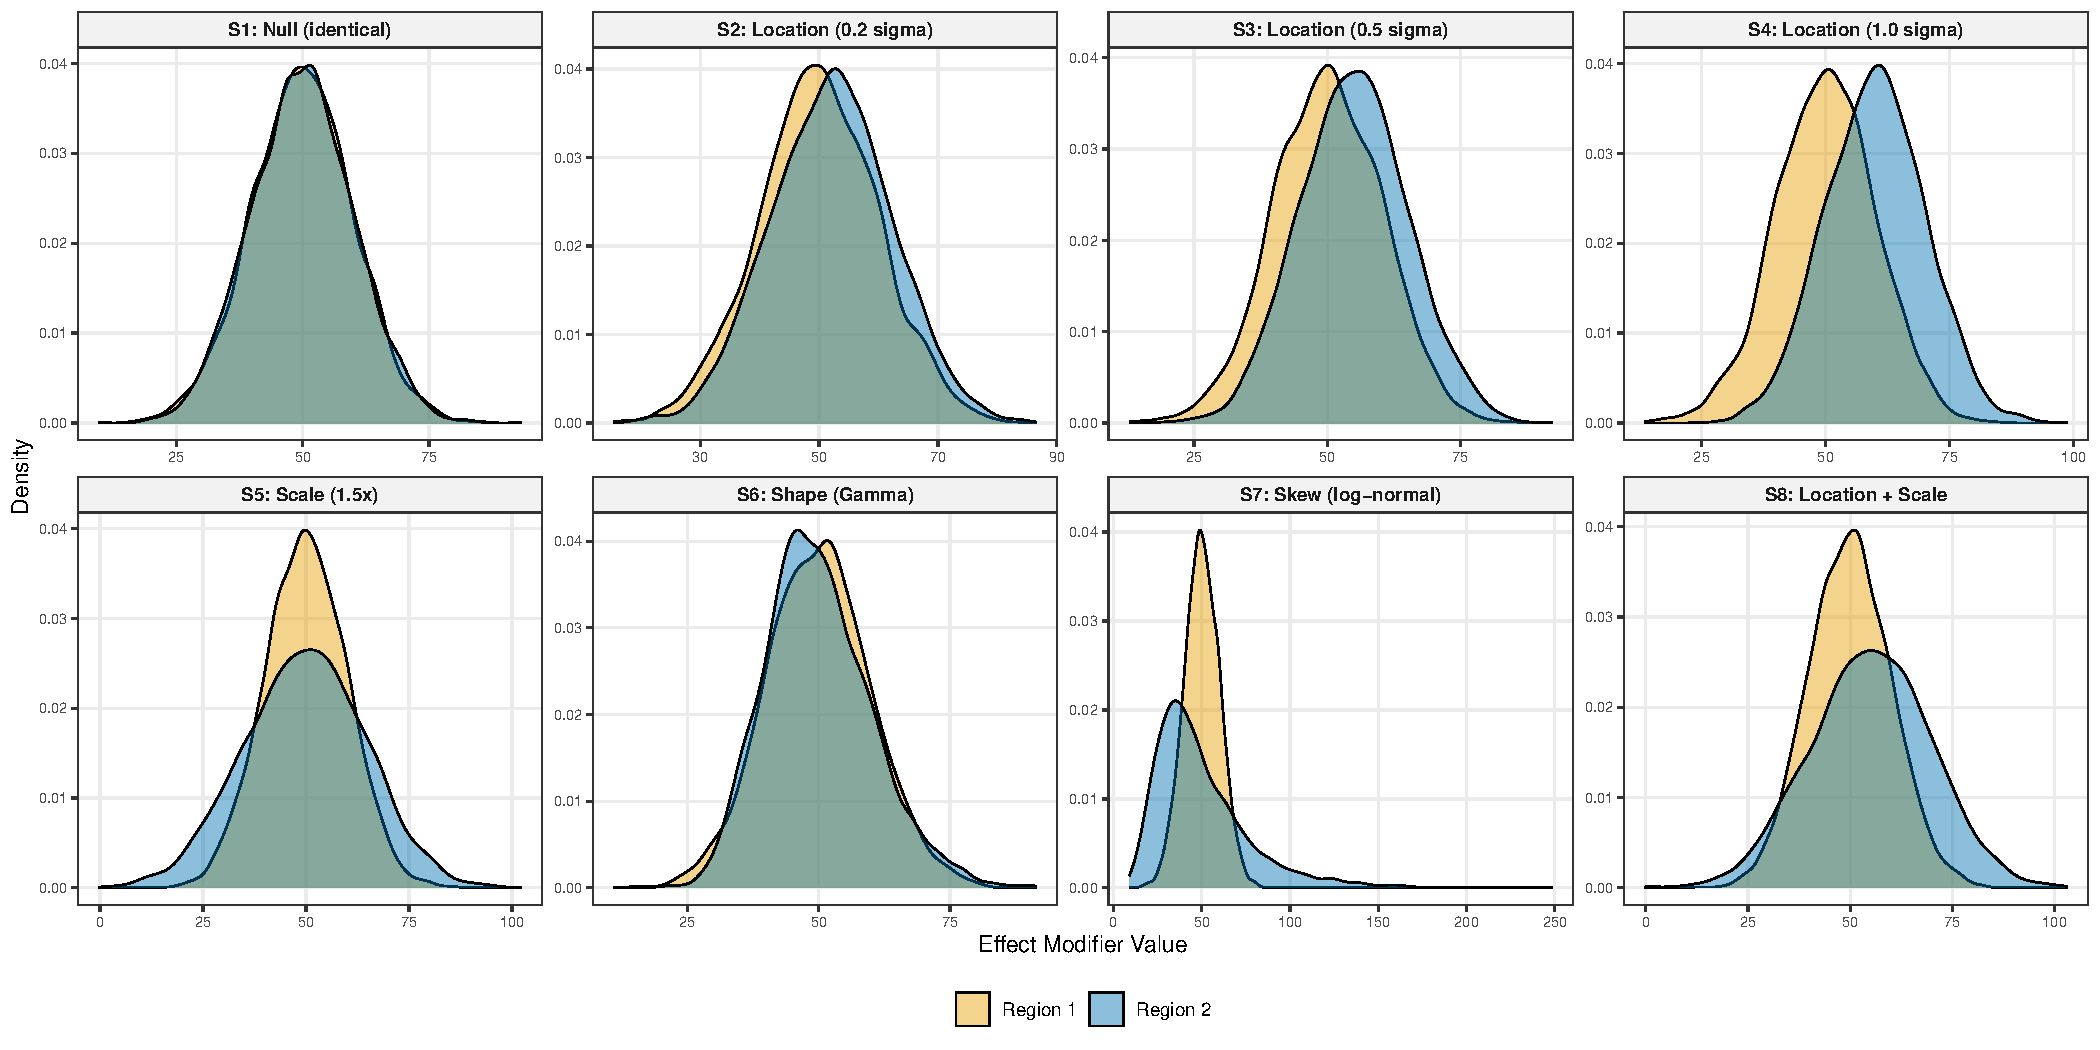
\includegraphics[width=0.95\linewidth]{fig1_scenario_overview.pdf}\\[2pt]
{\small\textit{Scenario overview: location, scale, and skew alterations
relative to the null reference.}}
\end{center}

\medskip
\centering\small
\renewcommand{\arraystretch}{1.05}
\begin{tabular}{@{}lll c@{}}
\toprule
\textbf{ID} & \textbf{Type} & \textbf{$F_1$ vs.\ $F_2$} & \textbf{True}\\
\midrule
S1 & Null             & $N(50,10^2)$ vs.\ same         & 0.000 \\
S2 & Loc.\ $0.2\sigma$& vs.\ $N(52,10^2)$              & 0.073 \\
S3 & Loc.\ $0.5\sigma$& vs.\ $N(55,10^2)$              & 0.180 \\
S4 & Loc.\ $1.0\sigma$& vs.\ $N(60,10^2)$              & 0.328 \\
S5 & Scale $1.5\times$& vs.\ $N(50,15^2)$              & 0.122 \\
S6 & Skew (LogN)      & vs.\ $\mathrm{LogN}(\mu,\sigma)$& 0.304 \\
S7 & Loc.\ + Scale    & vs.\ $N(55,15^2)$              & 0.175 \\
\bottomrule
\end{tabular}

\medskip
\raggedright
\textit{S7 is the most realistic MRCT pattern; S6 matches biomarker
CV$\approx 53\%$.}
\end{block}

\begin{block}{6.\ Estimation Quality: Bias \& Coverage}
Bias and 95\% percentile bootstrap CI coverage at $n=100$ per region:

\medskip
\begin{center}
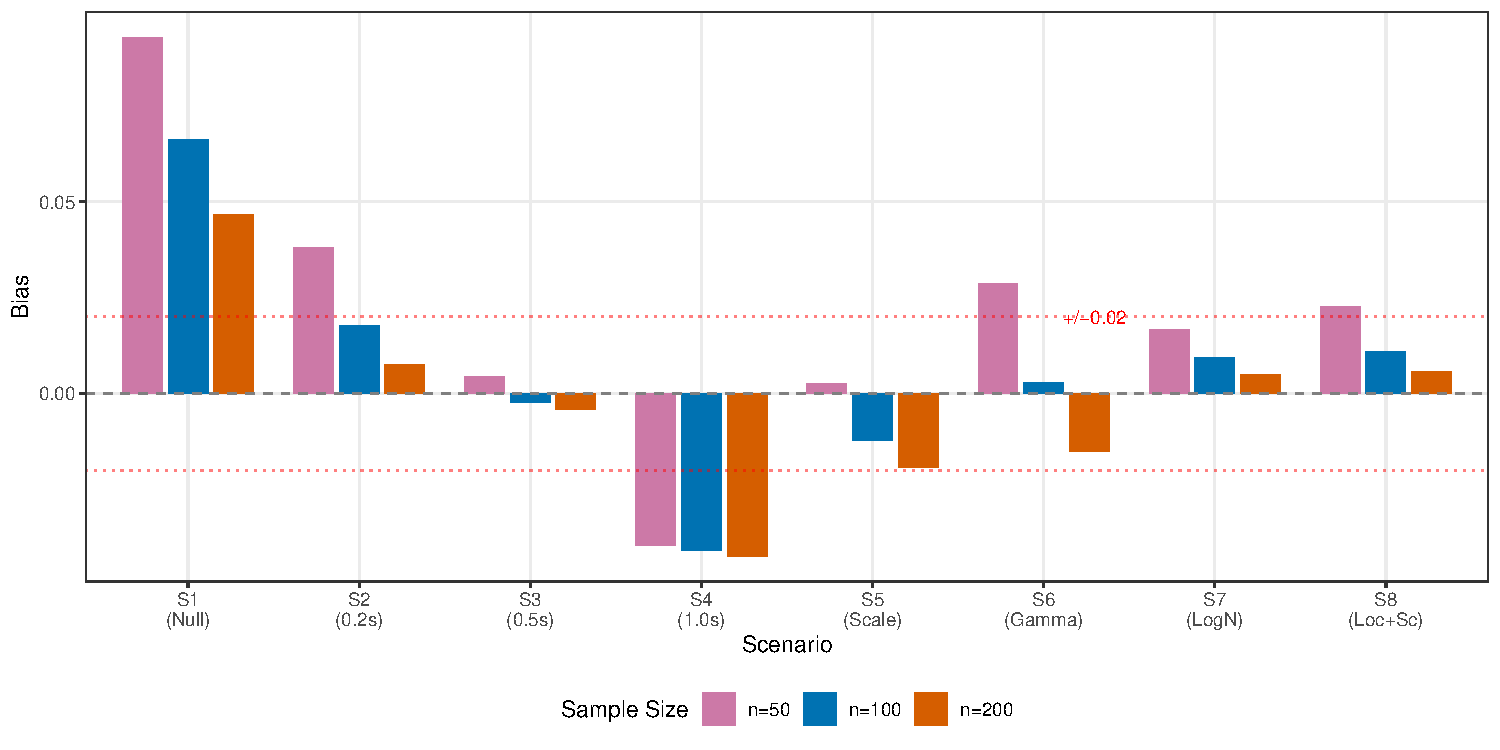
\includegraphics[width=0.95\linewidth]{fig3_bias.pdf}\\[2pt]
{\small\textit{Bias of $\hnABCD$ across scenarios and sample sizes.}}
\end{center}

\medskip
\centering\small
\begin{tabular}{@{}l c c c@{}}
\toprule
\textbf{Scenario} & \textbf{True} & \textbf{Bias} & \textbf{Coverage}\\
\midrule
S1 (Null)        & 0.000 & 0.066 & --\,\textsuperscript{\dag} \\
S2 (0.2$\sigma$) & 0.073 & 0.020 & 0.881                       \\
S3 (0.5$\sigma$) & 0.180 & 0.003 & \textbf{0.951}              \\
S4 (1.0$\sigma$) & 0.328 & 0.003 & \textbf{0.950}              \\
S5 (Scale)       & 0.122 & 0.014 & 0.910                       \\
S6 (Skew)        & 0.304 & 0.008 & \textbf{0.954}              \\
S7 (Loc+Scale)   & 0.175 & 0.011 & \textbf{0.935}              \\
\bottomrule
\end{tabular}

\medskip
\begin{center}
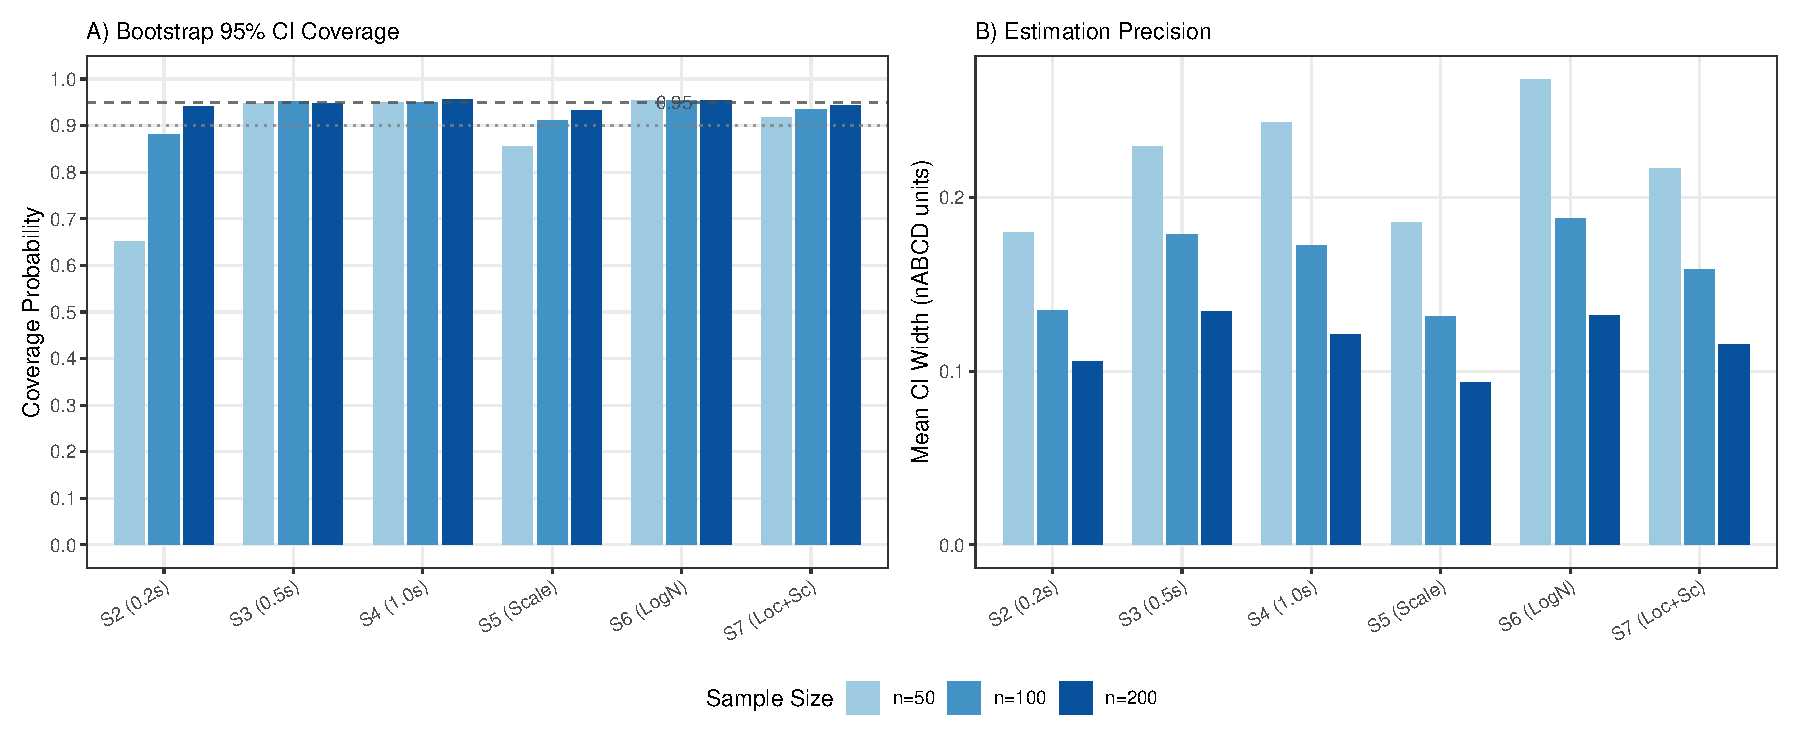
\includegraphics[width=0.95\linewidth]{fig4_estimation_quality.pdf}\\[2pt]
{\small\textit{Coverage and precision summary across scenarios.}}
\end{center}

\medskip
\raggedright\footnotesize
\textsuperscript{\dag}Near-boundary true value; non-negativity constraint
induces positive bias (Andrews, 2000).

\medskip
\raggedright\normalsize
\textbf{Take-aways.} True $\mathrm{nABCD}\geq 0.1$: bias $<0.02$, coverage
$0.88$--$0.96$ at $n\geq 100$. \textbf{Percentile} bootstrap preferred over
BCa.
\end{block}

\begin{block}{7.\ nABCD vs.\ SMD: Beyond Location}
At $n=100$ per region, SMD is blind to precisely the features that drive
non-linear effect-modifier heterogeneity:

\medskip
\centering\small
\begin{tabular}{@{}l c c l@{}}
\toprule
\textbf{Scenario} & \textbf{nABCD} & \textbf{SMD} & \textbf{Detected by}\\
\midrule
S3 Location & $0.183\pm 0.048$ & $0.50\pm 0.14$ & Both                       \\
S5 Scale    & $0.136\pm 0.033$ & $0.00\pm 0.14$ & \textbf{Only nABCD}        \\
S6 Skew     & $0.312\pm 0.048$ & $0.00\pm 0.14$ & \textbf{Only nABCD}        \\
\bottomrule
\end{tabular}

\medskip
\begin{center}
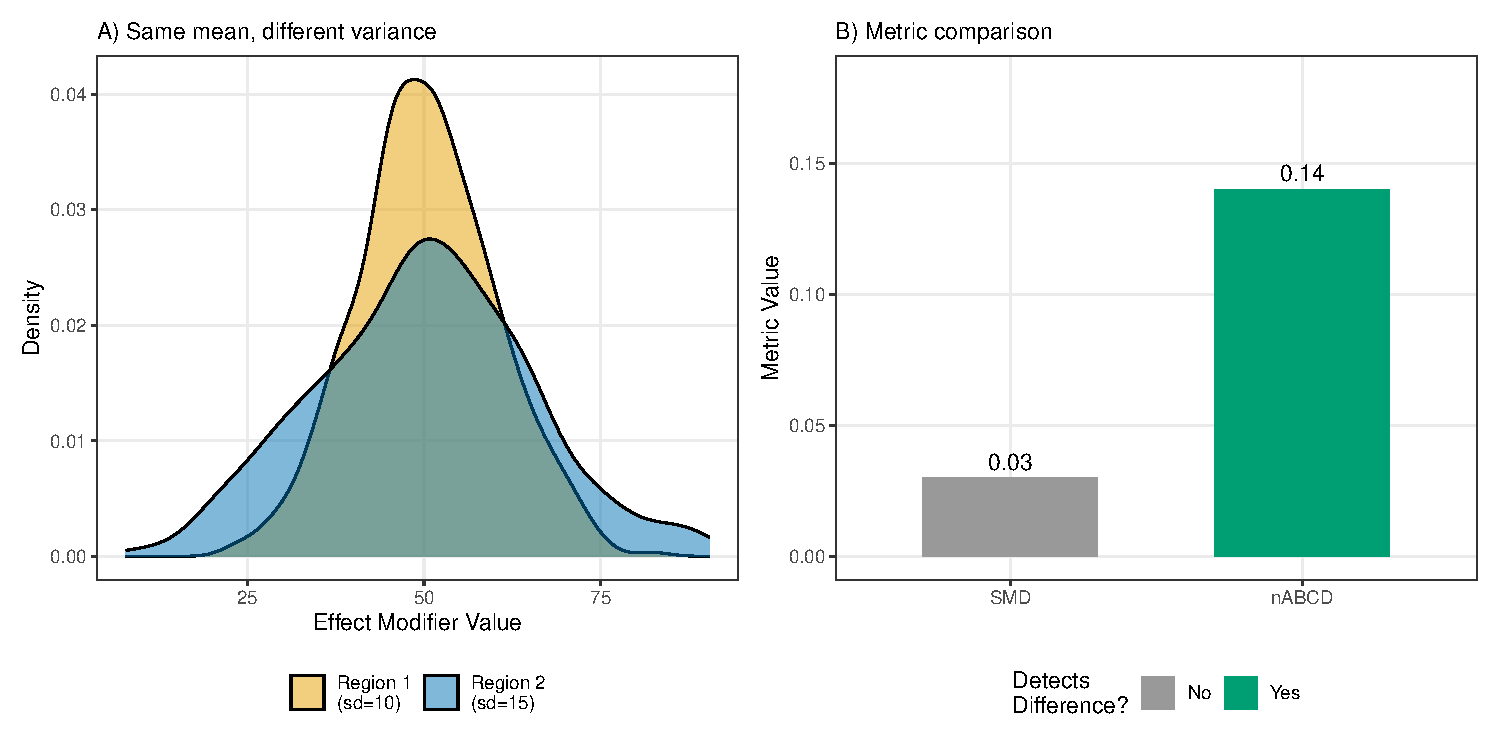
\includegraphics[width=0.95\linewidth]{fig5_smd_comparison.pdf}\\[2pt]
{\small\textit{nABCD detects scale and skew where SMD stays flat.}}
\end{center}

\medskip
\raggedright
\textbf{Framework philosophy.} Estimation-centered, not testing. Report
$\hnABCD$, bootstrap CI, and $\Delta_{\max}$ or $L^{*}$ -- never a binary
verdict. No universal cutoff: clinical weight depends on $L$, external to
the distributional comparison. ICH~E17 aligned.
\end{block}

\end{column}

%------------------------------------------------------------------------------
% COLUMN 3 (RIGHT) -- GUSTO-I application, conclusions, references
% Read order: 8 -> 9 -> 10 -> 11
%------------------------------------------------------------------------------
\begin{column}{0.325\textwidth}

\begin{block}{8.\ GUSTO-I Application: Drug T MRCT Planning}
A sponsor develops \textbf{Drug T}, a novel thrombolytic for acute myocardial
infarction, and plans a Phase~3 MRCT. At the planning stage the sponsor uses
IPD from \textbf{GUSTO-I} ($N=40{,}830$; 16 anonymized regions) to assess
distributional similarity of candidate effect modifiers across regions and to
identify pooling partners for a designated anchor region.

\medskip
\textbf{Candidate effect modifiers.} Age and systolic blood pressure (SBP),
flagged by Drug~T's Phase~2 exploratory analyses; class-level numerical CATE
slopes are unavailable. $L$ is therefore treated as unknown and the
$L^{*}$ pathway applies. \textbf{Region 8} is the anchor ($n=2{,}916$).

\medskip
\begin{center}
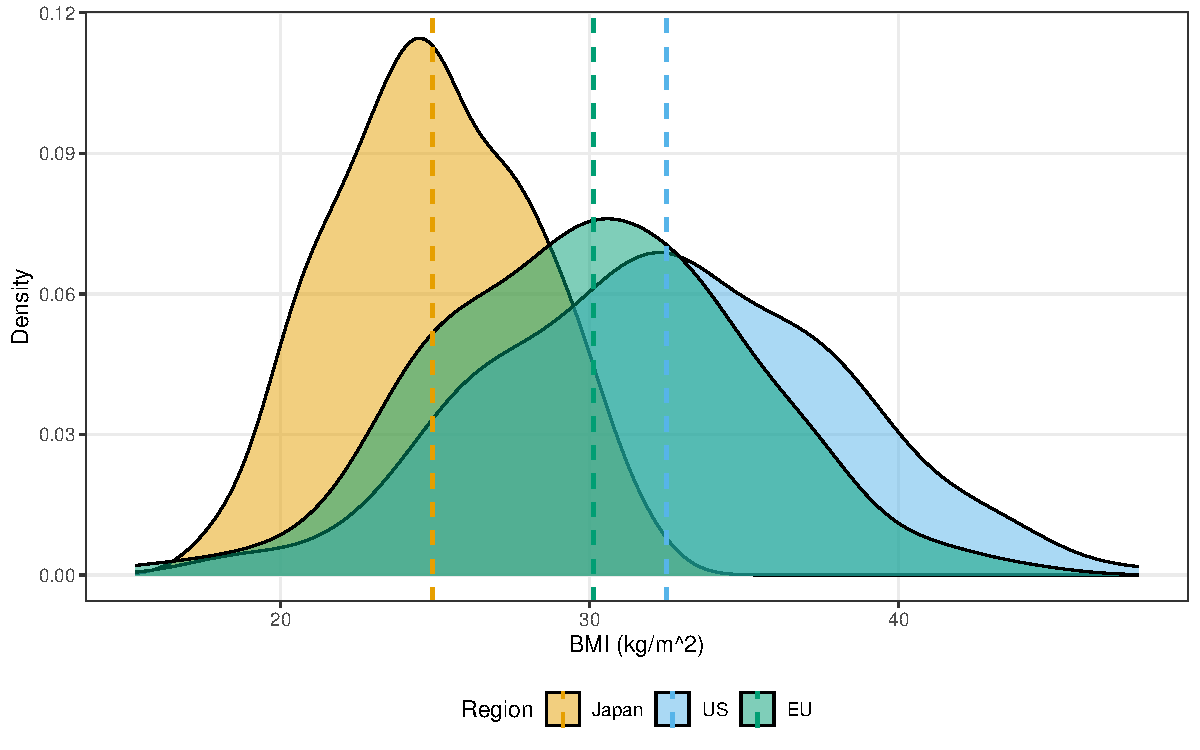
\includegraphics[width=0.95\linewidth]{fig6_application.pdf}\\[2pt]
{\small\textit{GUSTO-I anchor (R8) vs.\ partner regions: distributional
overview.}}
\end{center}

\medskip
\centering\small
\renewcommand{\arraystretch}{1.05}
\begin{tabular}{@{}clrll@{}}
\toprule
\textbf{Rank} & \textbf{Partner} & $n$ & \textbf{nABCD\textsubscript{age}} & \textbf{nABCD\textsubscript{SBP}}\\
\midrule
1  & R5 & 1909 & 0.011 [0.010, 0.026] & 0.056 [0.038, 0.077] \\
2  & R7 & 3150 & 0.011 [0.008, 0.026] & 0.082 [0.064, 0.098] \\
3  & R4 & 2876 & 0.016 [0.010, 0.032] & 0.042 [0.029, 0.060] \\
4  & R9 & 3123 & 0.017 [0.011, 0.032] & 0.110 [0.091, 0.130] \\
14 & R2 & 2952 & 0.061 [0.044, 0.079] & 0.015 [0.012, 0.030] \\
15 & R3 & 2030 & 0.076 [0.057, 0.095] & 0.051 [0.035, 0.074] \\
\bottomrule
\end{tabular}

\medskip
\begin{center}
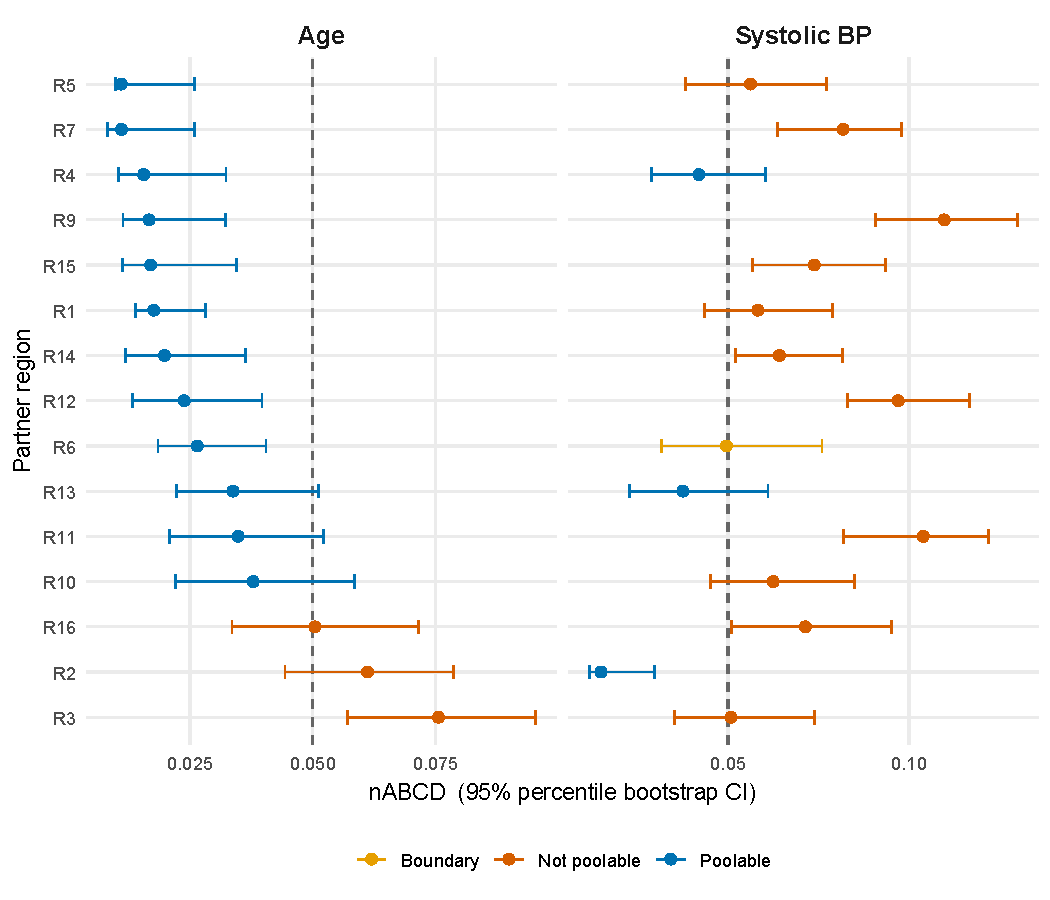
\includegraphics[width=0.95\linewidth]{fig_gusto_r8_forest.pdf}\\[1pt]
{\small\textit{Forest: nABCD with 95\% percentile bootstrap CIs
($B=2{,}000$).}}
\end{center}

\medskip
\begin{center}
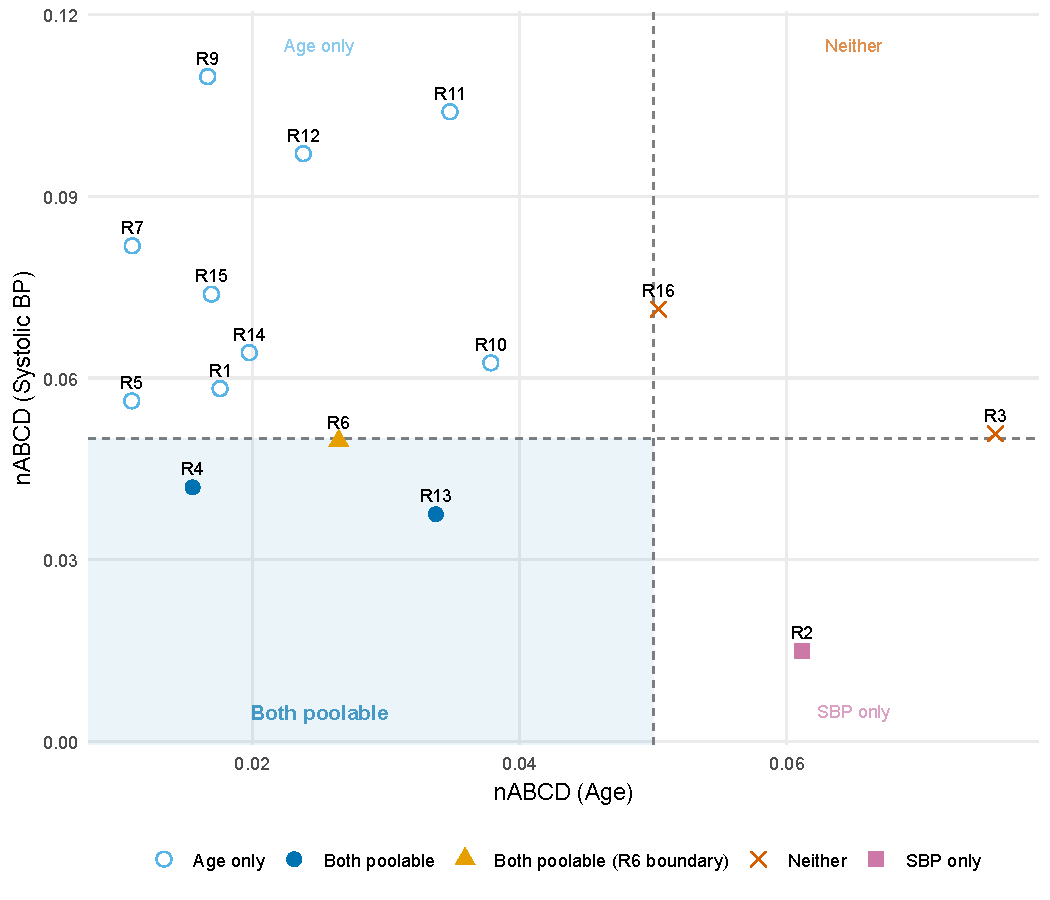
\includegraphics[width=0.95\linewidth]{fig_gusto_r8_scatter.pdf}\\[1pt]
{\small\textit{Joint view: lower-left favors pooling on both EMs.}}
\end{center}

\medskip
\raggedright
\textbf{R2 vs.\ R9 asymmetry.} R2 has the smallest SBP nABCD (0.015) but the
2nd-largest age nABCD (0.061); R9 shows the opposite. A single-modifier
ranking would draw opposite conclusions.

\medskip
\textbf{$L^{*}$ at $\Delta_{\text{clin}}=1$\%pt} (absolute 30-day mortality):
\centering\small
\renewcommand{\arraystretch}{1.05}
\begin{tabular}{@{}lcccc@{}}
\toprule
\textbf{Partner} & \textbf{nABCD\textsubscript{age}} & \textbf{nABCD\textsubscript{SBP}} & \textbf{$L^{*}$ age} & \textbf{$L^{*}$ SBP}\\
\midrule
R4  & 0.016 & 0.042 & \textbf{0.0180} & \textbf{0.0038} \\
R6  & 0.026 & 0.050 & \textbf{0.0110} & \textbf{0.0030} \\
R13 & 0.034 & 0.037 & \textbf{0.0087} & \textbf{0.0042} \\
R9  & 0.017 & 0.110 & 0.0171 & 0.0015 \\
R2  & 0.061 & 0.015 & 0.0047 & 0.0105 \\
\bottomrule
\end{tabular}

\medskip
\begin{center}

\includegraphics[width=0.95\linewidth]{fig_gusto_r8_calibration.pdf}\\[1pt]
{\small\textit{$L^{*}$ at $\Delta_{\text{clin}}=1$ and $2$\%pt.}}
\end{center}

\medskip
\raggedright
\textbf{Leading pooling candidates: R4, R6, R13.} They rank low on both
candidate EMs and their required $L^{*}$ values sit near the lower end of
the clinically plausible CATE-sensitivity range for thrombolysis in AMI.
The sponsor may reasonably prioritize these regions for pooling with R8.
\end{block}

\begin{block}{9.\ Conclusions \& Implications}
\begin{enumerate}
  \item \textbf{nABCD} captures full distributional differences (location,
        scale, shape, skew) that SMD misses by construction.
  \item The heterogeneity bound
        $|\bar\tau_1-\bar\tau_2|\leq 2L\cdot\mathrm{IQR}_{\text{pooled}}\cdot\mathrm{nABCD}$
        translates distributional distance into a clinical-scale bound --
        a property unique to $W_1$.
  \item Seven-scenario simulation: bias $<0.02$, coverage $0.88$--$0.96$ for
        true $\mathrm{nABCD}\geq 0.1$ at $n\geq 100$.
  \item GUSTO-I illustration: ranking + CIs + $L^{*}$ identify R4/R6/R13 as
        leading pooling candidates for R8, while exposing the R2 vs.\ R9
        asymmetry that single-modifier rankings would obscure.
  \item Fills a methodological gap in ICH~E17 implementation by supplying
        \emph{transparent quantitative inputs} without imposing a universal
        cutoff.
\end{enumerate}

\medskip
\textbf{Limitations.} Continuous, univariate effect modifiers (multivariate
OT extension is future work); near-boundary positive bias for true
$\mathrm{nABCD}\lesssim 0.05$; requires representative baseline data.

\medskip
\textbf{Available.} R code for nABCD and bootstrap inference; an R package
is under development.
\end{block}

\begin{block}{10.\ Key References}
\footnotesize
\begin{list}{[\arabic{enumi}]}{\usecounter{enumi}\setlength{\leftmargin}{2em}\setlength{\itemsep}{1pt}\setlength{\parsep}{0pt}\setlength{\topsep}{2pt}}
  \item ICH~E17 EWG (2017). \textit{General Principles for Planning and
        Design of MRCTs}.
  \item Matsushima N, et al.\ (2024) \textit{Clin Pharmacol Ther}
        115:965--970. doi:10.1002/cpt.3163.
  \item Song J, et al.\ (2025) \textit{Ther Innov Regul Sci} 59:359--364.
        doi:10.1007/s43441-025-00744-8.
  \item Villani C (2009). \textit{Optimal Transport: Old and New}. Springer.
        doi:10.1007/978-3-540-71050-9.
  \item Panaretos VM, Zemel Y (2019) \textit{Annu Rev Stat Appl} 6:405--431.
        doi:10.1146/annurev-statistics-030718-104938.
  \item del Barrio E, Gin\'e E, Matr\'an C (1999) \textit{Ann Probab}
        27:1009--1071. doi:10.1214/aop/1022677394.
  \item Sommerfeld M, Munk A (2018) \textit{JRSS-B} 80:219--238.
        doi:10.1111/rssb.12236.
  \item Gibbs AL, Su FE (2002) \textit{Int Stat Rev} 70:419--435.
        doi:10.1111/j.1751-5823.2002.tb00178.x.
  \item GUSTO Investigators (1993) \textit{N Engl J Med} 329:673--682.
        doi:10.1056/NEJM199309023291001.
  \item FTT Collaborative Group (1994) \textit{Lancet} 343:311--322.
        doi:10.1016/S0140-6736(94)91161-4.
  \item Andrews DWK (2000) \textit{Econometrica} 68:399--405.
        doi:10.1111/1468-0262.00114.
  \item Wasserstein RL, Lazar NA (2016) \textit{Am Stat} 70:129--133.
        doi:10.1080/00031305.2016.1154108.
\end{list}
\end{block}

\begin{block}{11.\ Acknowledgments \& Contact}
\small
The authors thank colleagues for methodological discussions and the GUSTO-I
investigators for making de-identified IPD available for methodological
research.

\medskip
\centering\small\color{midgray}
Correspondence: corresponding@institution.edu \quad\textbullet\quad
R code available on request \quad\textbullet\quad
Manuscript submitted to \textit{Statistics in Medicine}.
\end{block}

\end{column}

\end{columns}

\end{frame}

\end{document}
